\documentclass[../structure.tex]{subfiles}
%\usepackage{../mypkg}
\begin{document}
\chapter{Introduction}

	The human brain, which is the focus of our work in this thesis, is the central organ of the human nervous system. It is made up of two main components, namely, gray 	     			    matter and white matter. Researchers have discerned a great deal about gray and white matter and distinct brain regions through autopsies and imaging techniques. The study 		of the human brain in diseased states or under conditions associated with brain damage have resulted in major insights into this complex organ.

\section{Brain Anatomy :Fiber Pathways}

	 \textbf{White matter} refers to areas of the central nervous system that are mainly made up of myelinated axons, also called tracts or fiber pathways \cite{Blumenfeld2010}. It is composed of bundles which connect various gray matter areas of the brain to each other and carry nerve impulses between neurons. Myelin acts as an insulator allowing electrical signals to jump rather than course through axons, increasing the speed of transmission of all nerve signals through a phenomenon known as saltatory conduction \cite{Klein2008}.
	\\Long thought to be passive tissue, white matter affects learning and brain functions, modulates the distribution of action potentials, and acts as a relay and coordinator of communication between different brain regions \cite{Fields2008}.
	
	The human brain consists of the following tracts on the left and right sides:
	\begin{comment}
   \begin{itemize}
       \item Anterior Thalamic Radiation (ATR)
       \item Corpus Callosum (CC)
       \item Genu of the Corpus Callosum (genu)
       \item Splenium of the Corpus Callosum (splenium)
       \item Body of Corpus Callosum (truncus)
		\item Cingulum (Cing)
		\item Corticospinal Tract (CST)
		\item Inferior Fronto-occipital Fasciculus (IFO)
		\item Inferior Longitudinal Fasciculus (ILF)
		\item Superior Longitudinal Fasciculus (SLF)
		\item Ventral Tegmental Area (VTA)
	\end{itemize}
	\end{comment}

	\begin{figure}[h!]
	\centering
	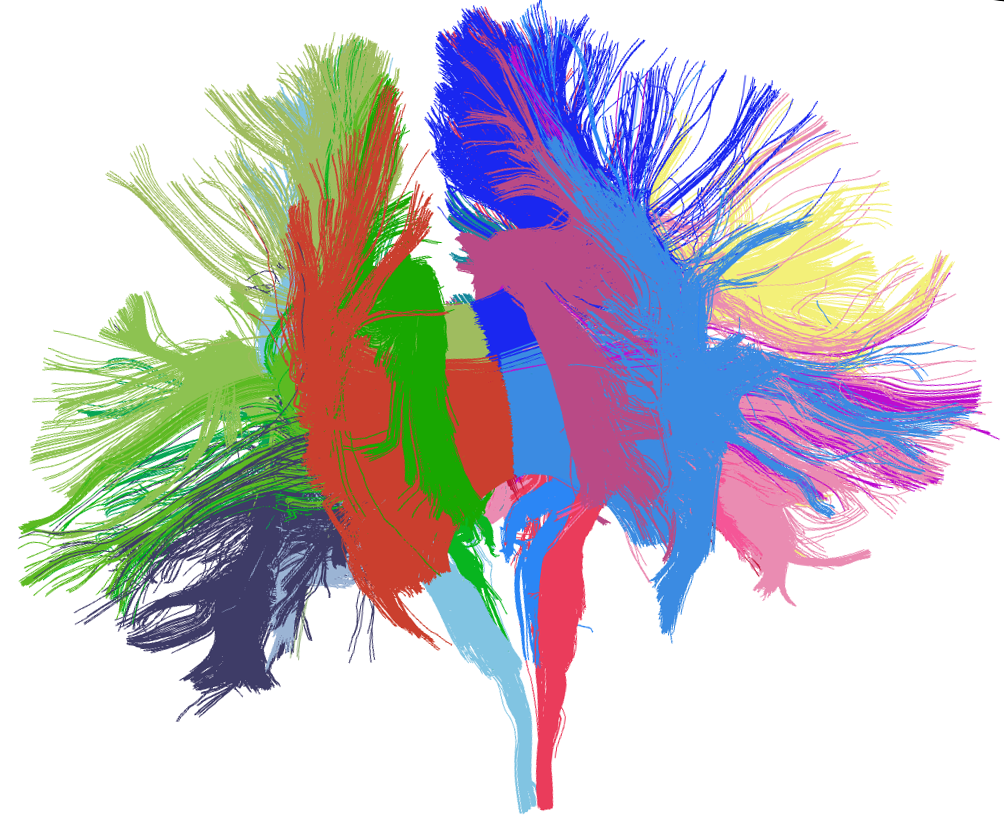
\includegraphics[scale=0.4]{000_all_brain}
	\captionsetup{justification=centering}
	\caption{The Human Brain Fiber Pathway}
	\label{fig:all_brain}
	\end{figure}
	
	\textbf{Thalamic Radiation (ATR)}
		refers to fiber pathways that connect the anterior nuclear group of the thalamus and the midline nuclear group of the thalamus with the frontal lobe through the anterior thalamic peduncle, the anterior limb of the internal capsule and other parts of the cerebral white matter \cite{Washington1994}\cite{Grimm2018}. ATR abnormalities have a possible link with cognitive abnormalities and negative symptoms in schizophrenia\cite{Mamah2010}.
		
		\textbf{Corpus Callosum (CC)} 
		is a wide, flat bundle of nerve fibers, located at the longitudinal fissure beneath the cortex, which acts a link between the two hemispheres of the brain and facilitates communication between them. The term corpus callosum means 'tough body' in Latin. With approximately 200 - 250 million contralateral axonal projections to its credit, it is the largest among the various white matter structures in the central nervous system.
The anterior portion of this structure is called '\textit{genu}', while the posterior structure is called '\textit{splenium}'. In between its anterior and posterior portions, lies the 'truncus' or its '\textit{body}'. Studies have revealed that the anterior of corpus callosum in left-handed people is eleven percent (100\%) larger than that of right-handed people \cite{PDD2015}.
		
		\textbf{Genu of the Corpus Callosum (genu)} 
		refers to the rostral most portion of the corpus callosum. It is bounded caudally by the body of the corpus callosum and ventrocaudally by the rostrum of the corpus callosum \cite{Washington1994}.
		
		\textbf{Splenium of the Corpus Callosum (splenium)}
		 refers to the caudal most portion of the corpus callosum. It is bounded rostrally by the body of the corpus callosum \cite{Washington1994}.
It overlaps the tela chorioidea of the third ventricle and the mid-brain, and ends in a thick, convex, free border. A sagittal section of the splenium shows that the posterior end of the corpus callosum is acutely bent forward, the upper and lower parts being applied to each other \cite{PDD2015}.

\textbf{Body of Corpus Callosum (truncus)} 
		 refers to the portion of the corpus callosum located between the genu of the corpus callosum and the splenium of the corpus callosum. In a common parcellation, corpus callosum, it is divided into four parts: the rostral body of the corpus callosum, the anterior midbody of the corpus callosum, the posterior midbody of the corpus callosum and the isthmus of the corpus callosum \cite{Washington1994}.
		\textbf{Cingulum (Cing)}
		refers to a fiber pathway that runs longitudinally in the cingulate white matter; it connects portions of the cingulate gyrus, the parietal lobe and the prefrontal cortex with the parahippocampal gyrus and adjacent structures of the temporal lobe. "All connectios entering and exiting the cingulate gyrus pass through the cingulum bundle". It is composed of the Cingulum ammonale and the Cingulum limitans \cite{Washington1994}.\\
		
	\begin{comment}
		%In neuroanatomy, the cingulum is a collection of white matter fibers projecting from the cingulate gyrus to the entorhinal cortex in the brain, allowing for communication between components of the limbic system. It forms the white matter core of the cingulate gyrus, following it from the subcallosal gyrus of the frontal lobe beneath the rostrum of corpus callosum to the parahippocampal gyrus and uncus of the temporal lobe.
Cingulum receives afferent fibers from the parts of the thalamus that are associated with the spinothalamic tract. This, in addition to the fact that the cingulum is a central structure in learning to correct mistakes, indicates that the cingulum is involved in appraisal of pain and reinforcement of behavior that reduces it \cite{Brodal2016}.
%Cingulotomy, the surgical severing of the anterior cingulum, is a form of psychosurgery used to treat depression and OCD.
%The cingulum was one of the earliest identified brain structures.
%Anatomy and Function
The cingulum is described from various brain images as a C shaped structure within the brain that wraps around the frontal lobe to the temporal lobe right above the corpus callosum. It is located beneath the cingulate gyrus within the medial surface of the brain therefore encircling the entire brain. There are two primary parts of the cingulate cortex, as is typical with most brain structures. There is the posterior cingulate and anterior cingulate. The anterior is linked to emotion, especially apathy and depression. Here function and structure changes are related meaning any change within this structure would lead to a function change, particularly behavioral because of its function involving emotions. Damage to this area can have various effects on mental disorders and mental health. The posterior section is more related to cognitive functions. This can include attention, visual and spatial skills, working memory and general memory. Because of its location, the cingulum is very important to brain structure connectivity and the integration of information that it receives \cite{JaredTanner2010}.
	\end{comment}
	\textbf{Corticospinal Tract (CST)}
		refers to a fiber pathway from the cerebral cortex to the spinal cord. Its fibers originate from pyramidal neurons of the precentral gyrus, and on their way to the spinal cord, they pass through parts of the cerebral white matter (including the posterior limb of the internal capsule), the crus cerebri, the longitudinal pontine fibers, the pyramid of the medulla (where they are known as the pyramidal tract) and the pyramidal decussation. In the ducussation, some fibers cross to the other side of the brainstem to form the lateral corticospinal tract. Those fibers that do not cross split to form the anterolateral corticospinal tract and the anterior corticospinal tract \cite{Washington1994}.
		
		\textbf{Fornix (Fornix)}
		The fornix (Latin, "vault" or "arch") is a C-shaped bundle of fibers (axons) in the brain, and carries signals from the hippocampus to the hypothalamus.
The fibres begin in the hippocampus on each side of the brain (where they are also known as the fimbria); the separate left and right sides are each called the crus of the fornix. The bundles of fibres come together in the midline of the brain, forming the body of the fornix. The inferior edge of the septum pellucidum (a membrane that separates the two lateral ventricles) is attached to the upper face of the fornix body.
The body of the fornix travels anteriorly and divides again near the anterior commissure. The left and right parts separate, but there is also an anterior/posterior divergence.
The posterior fibres (called the postcommissural fornix) of each side continue through the hypothalamus to the mammillary bodies; then to the anterior nuclei of thalamus, which project to the cingulate cortex.
The anterior fibers (precommissural fornix) end at the septal nuclei and nucleus accumbens of each half of the brain \cite{PDD2015}.

		While its exact function and importance in the physiology of the brain are still not entirely clear, it has been demonstrated that surgical transection – the cutting of the fornix along its body – can cause memory loss \cite{HenryGray1918}. There is some debate over what type of memory is affected by this damage, but it has been found to most closely correlate with recall memory rather than recognition memory. This means that damage to the fornix can cause difficulty in recalling long-term information such as details of past events, but it has little effect on the ability to recognize objects or familiar situations \cite{HenryGray1918}.
		
		\textbf{Inferior Fronto-occipital Fasciculus (IFO)}
		The occipitofrontal fasciculus passes backward from the frontal lobe, along the lateral border of the caudate nucleus, and on the medial aspect of the corona radiata; its fibers radiate in a fan-like manner and pass into the occipital and temporal lobes lateral to the posterior and inferior cornua \cite{PDD2015}.
		
		\textbf{Inferior Longitudinal Fasciculus (ILF)}
		The inferior longitudinal fasciculus connects the temporal lobe and occipital lobe, running along the lateral walls of the inferior and posterior cornua of the lateral ventricle.
The existence of this fasciculus independent from the occipitotemporal fasciculus has been questioned for the human being, such that it has been proposed that the term inferior longitudinal fasciculus be replaced by the term "occipitotemporal projection" \cite{PDD2015}.

		\textbf{Superior Longitudinal Fasciculus (SLF)}
		refers to a fiber pathway in the cerebral white matter. It is composed of fibers that connect the cortex of the frontal lobe with cortex of the occipital lobe and the temporal lobe. Some authors refer to the connection with the temporal lobe as the arcuate fasciculus \cite{Washington1994}.
		
		is a pair of long bi-directional bundles of neurons connecting the front and the back of the cerebrum. Each association fiber bundle is lateral to the centrum ovale of a cerebral hemisphere and connects the frontal, occipital, parietal, and temporal lobes. The neurons pass from the frontal lobe through the operculum to the posterior end of the lateral sulcus where numerous neurons radiate into the occipital lobe and other neurons turn downward and forward around the putamen and radiate to anterior portions of the temporal lobe \cite{PDD2015}.
		
		\textbf{Ventral Tegmental Area (VTA)}
		After substantia nigra, VTA which is situated adjacent to the substantia nigra in the midbrain is one of the major dopaminergic areas in the brain. Even though there is no clear anatomical separation between the two, there are areas that seem to differ slightly.

Together with an integral part of a network of structures, it is known as the reward system involved in reinforcing behavior. VTA is also thought to play major role in motivation, reward, emotional and cognitive processes. VTA is activated with experiencing something rewarding which may be necessary to the development of addiction. 

Other than addiction VTA is involved in pathophysiology of disorders as in case of schizophrenia where dopaminergic neurons in the VTA have been proposed to play a role and attention-deficit hyperactivity disorder (ADHD) has been linked to low dopamine activity in the VTA \cite{Kalivas1993}.
	
	
\section{Registration}
	The registration problem or sometimes called alignment or absolute orientation is one of fundamental problem in computer vision. If we have two objects and we need to align them that means we should reduce the distance between them by making one object fix and move the other one to the closest distance, this simple form of alignment called rigid transformation, if we add scaling then it call non-rigid transformation and it will extend the size of the object as well. Due to its fundamental importance in computer vision, it is necessary step in many different applications, for instance: object recognition, tracking, range data fusion, graphics, medical image alignment, robotics and structural bioinformatics etc \cite{Li2007}.
		\subsection{Iterative closest point (ICP)}
		 ICP, which is an algorithm employed to minimize the distance between two or more points clouds, is one of the most widely used algorithms in aligning three objects with initial position \cite{Zhang1994}.
		 In ICP (in our case) one points cloud (i.e., vertex cloud), or target, is kept fixed, while the template, is transformed to best match the target. The algorithm iteratively check the transformation (combination of translation, rotation and scaling) required to minimize a distance from the template to the target points cloud.
\section{Principal component analysis}
%PCA is mathematically defined as an orthogonal linear transformation that transforms the data to a new coordinate system such that the greatest variance by some projection of the data comes to lie on the first coordinate (called the first principal component), the second greatest variance on the second coordinate, and so on\cite{Jolliffe2002}.
PCA is used in the code as a preliminary step, so that the template and target are aligned as much as possible before the registration can begin.
\section{Least squares (LSQR)}
LSQR is linear iterative method to find the value of $x$ by solving the equation $||Ax-b||^2$.
%LSQR uses an iterative method to approximate the solution. The number of iterations required to reach a certain accuracy depends strongly on the scaling of the problem ($ ||Ax-b||^2 $). Poor scaling of the rows or columns of A should therefore be avoided where possible \cite{Paige1982}.
\end{document}

